\section{\textlatin{UI/UX}}
Η σχεδίαση του \textlatin{UI/UX} έγινε έτσι ώστε ο χρήστης, δηλαδή ο μαθητής που θα μπει στην σελίδα, να μπορεί να πλοηγείται με ευκολία και οργάνωση. Η πλοήγηση του μαθητή θα γίνεται σειριακά. Συγκεκριμένα:

\begin{itemize}
    \item Ο μαθητής θα αρχίζει κάνοντας \textbf{\textlatin{Login}} στην αρχική φόρμα που θα του εμφανίζεται (την πρώτη φορά που θα επισκεφτεί την σελίδα θα πρέπει να δημιουργήσει τον λογαριασμό του χρησιμοποιώντας την αντίστοιχη φόρμα \textbf{\textlatin{Register}}.
\end{itemize}
\begin{figure}[H]
        \centering
        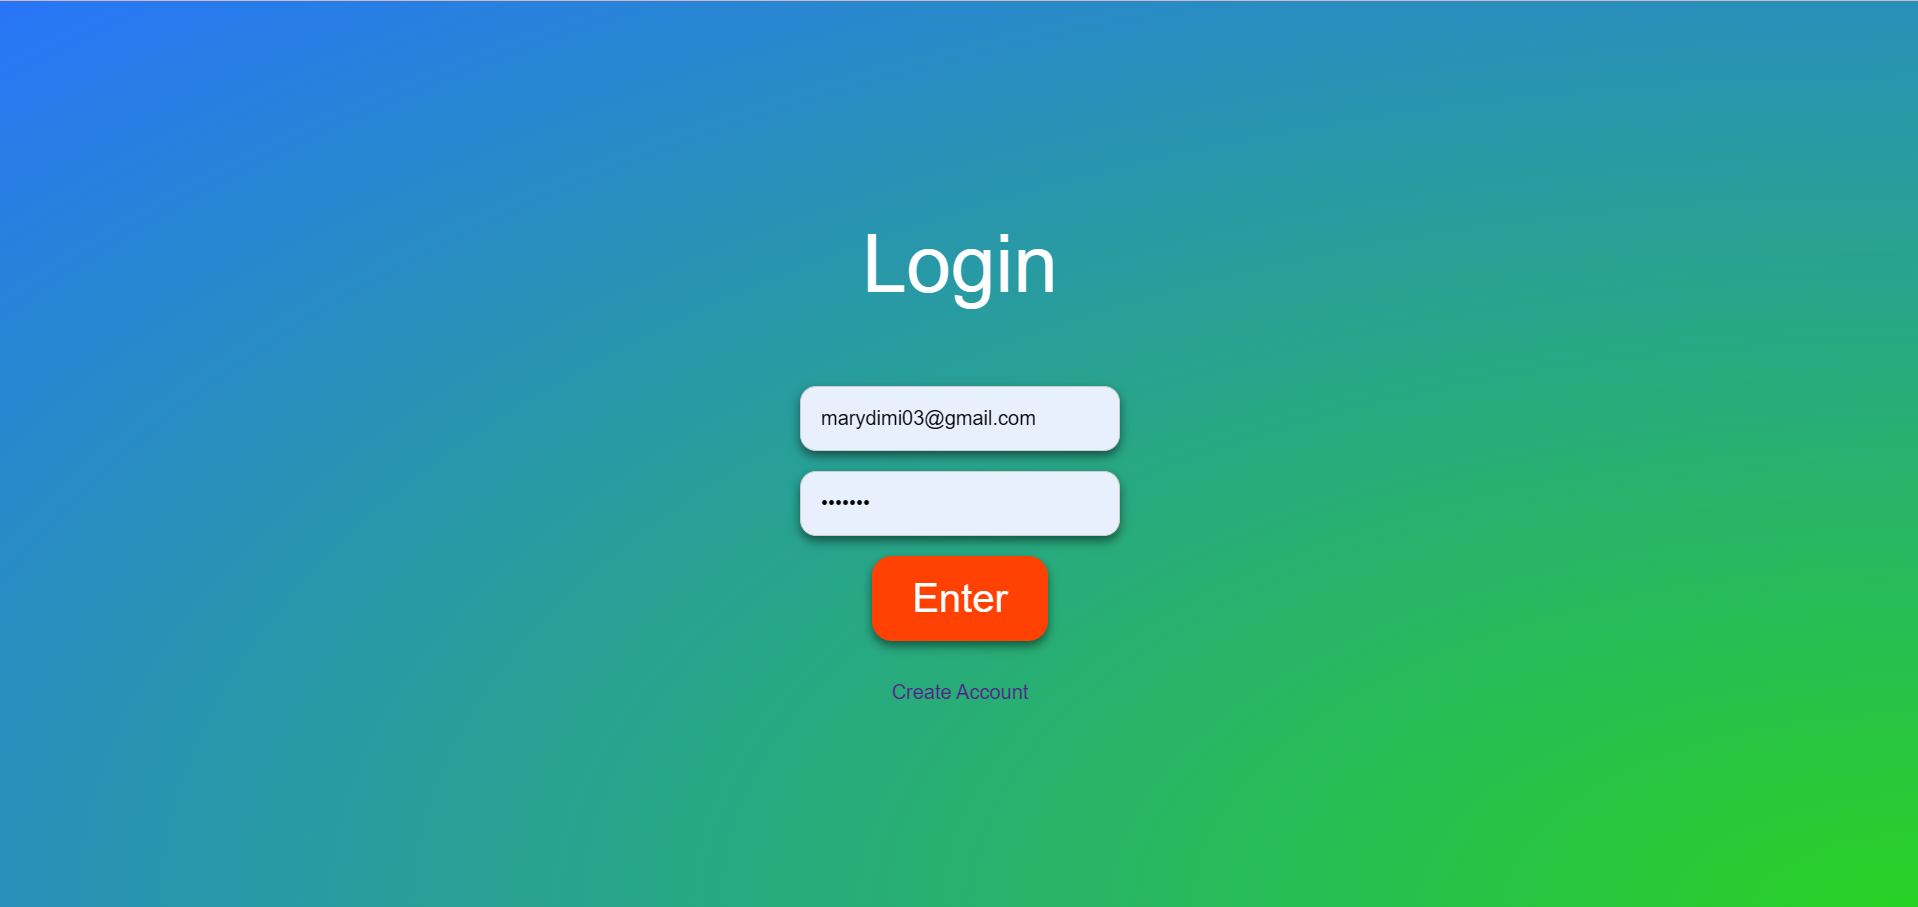
\includegraphics[width=1\linewidth]{img/Login.png}
        \caption{\textlatin{Login Page}}
\end{figure}
\begin{figure}[H]
    \centering
    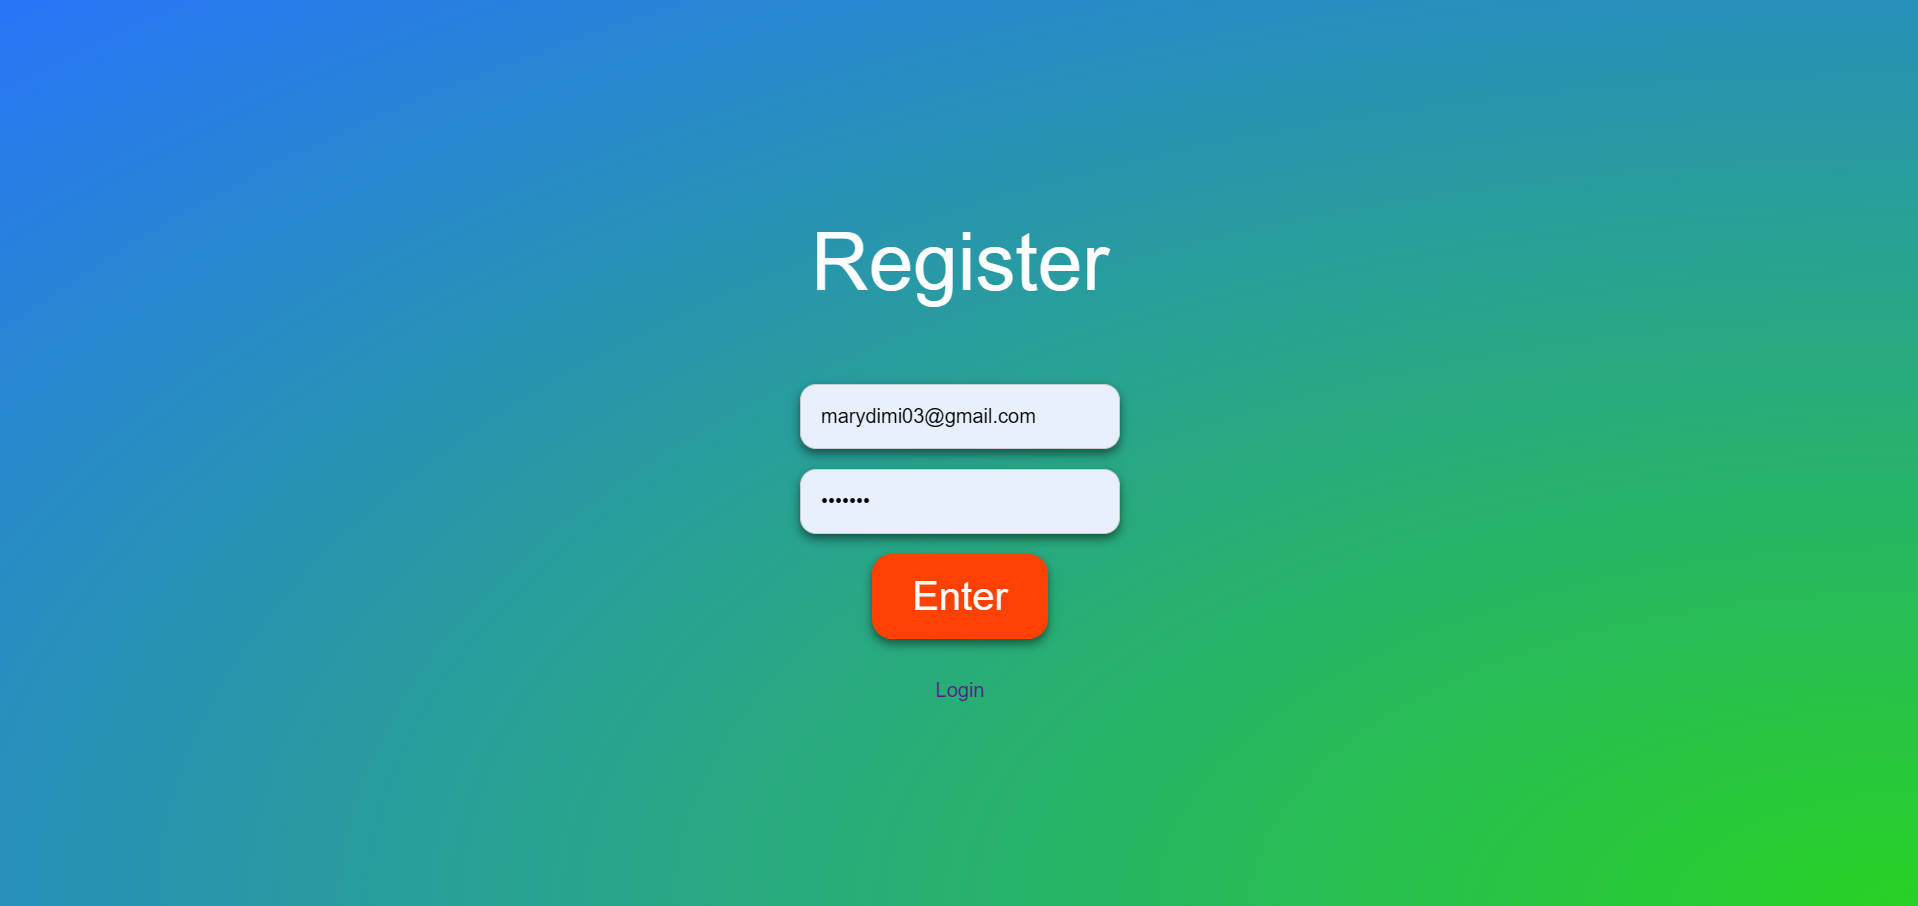
\includegraphics[width=1\linewidth]{img/Register.png}
    \caption{\textlatin{Register Page}}
\end{figure}

\newpage

\begin{itemize}
    \item Στην συνέχεια θα ακολουθεί το \textbf{κεντρικό μενού,} με τις επιλογές να αρχίσει ή να συνεχίσει την πρόοδο του (\textbf{\textlatin{Learn/Continue}}), εφόσον το λογισμικό θα "θυμάται" που έχει μείνει ο κάθε μαθητής, και η άλλη θα είναι να δει τα στατιστικά του (\textbf{\textlatin{Statistics}}), δηλαδή με πιο απλά λόγια τις επιδόσεις του στις δραστηριότητες που έχει ολοκληρώσει (\textlatin{quizzes, exam}).
\end{itemize}
\begin{figure}[H]
    \centering
    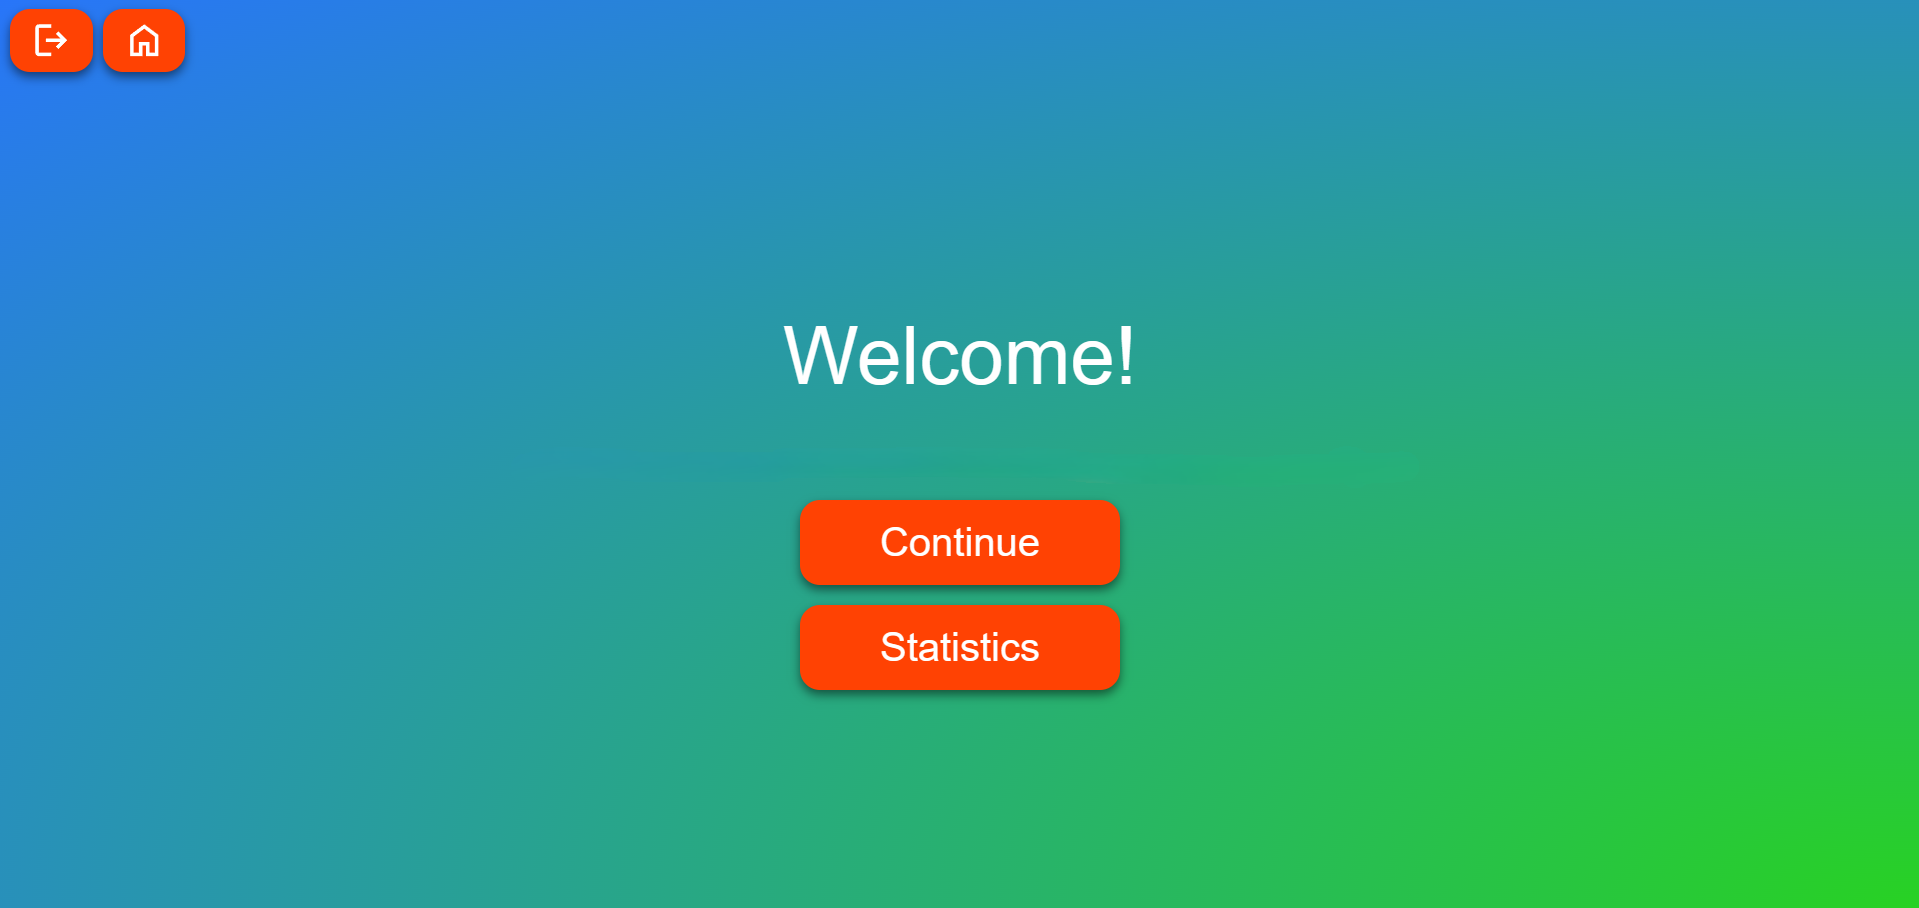
\includegraphics[width=1\linewidth]{img/Menu.png}
    \caption{\textlatin{Menu Page}}
\end{figure}

\begin{itemize}
    \item Παρακάτω βλέπουμε τα κεφάλαια της θεωρίας (\textlatin{\textbf{History, Geography, Culture}}). Ο μαθητής καλείται να τα διαβάσει και να τα αποστηθίσει όσο καλύτερα μπορεί, προκειμένου να βρίσκεται σε θέση να απαντήσει τα quizzes που ακολουθούν, έπειτα από κάθε κεφάλαιο. Τα κεφάλαια χωρίζονται σε ενότητες με σκοπό την διευκόλυνση του μαθητή κατά την διάρκεια της εκμάθησης τους.
\end{itemize}
\begin{figure}[H]
    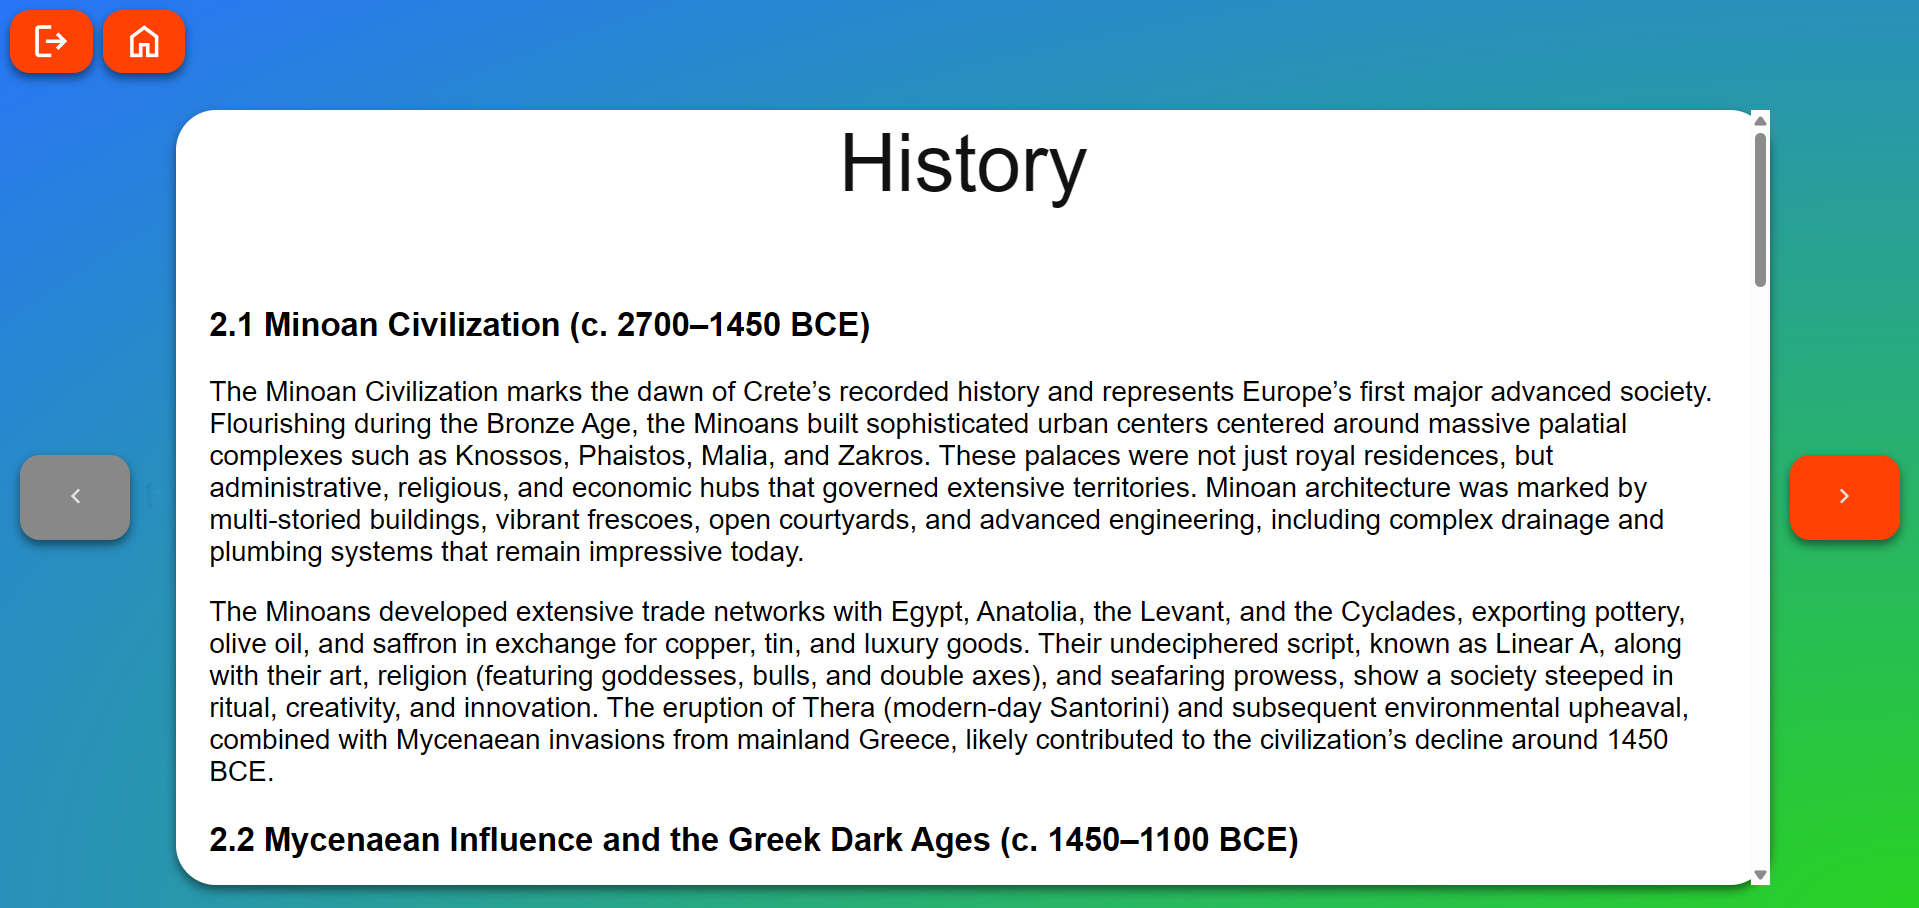
\includegraphics[width=0.5\linewidth]{img/Theory-History.png}
     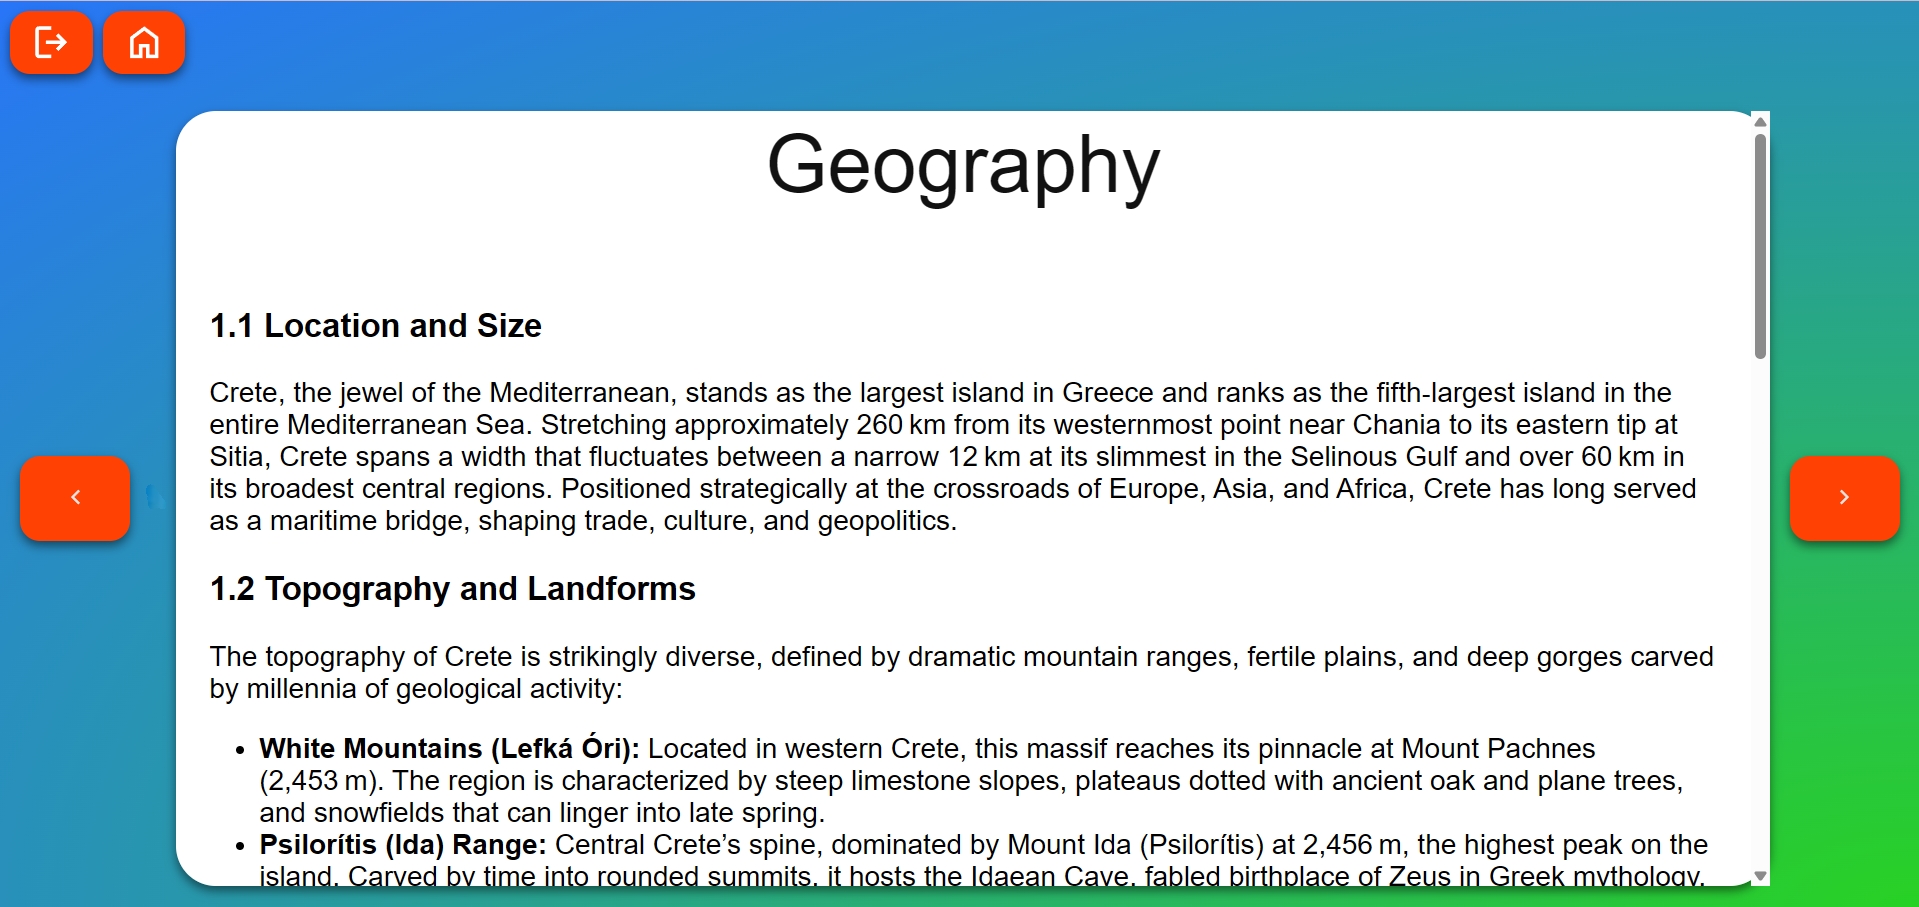
\includegraphics[width=0.5\linewidth]{img/Theory-Geography.png}
\end{figure}
\begin{figure}[H]
    \centering
    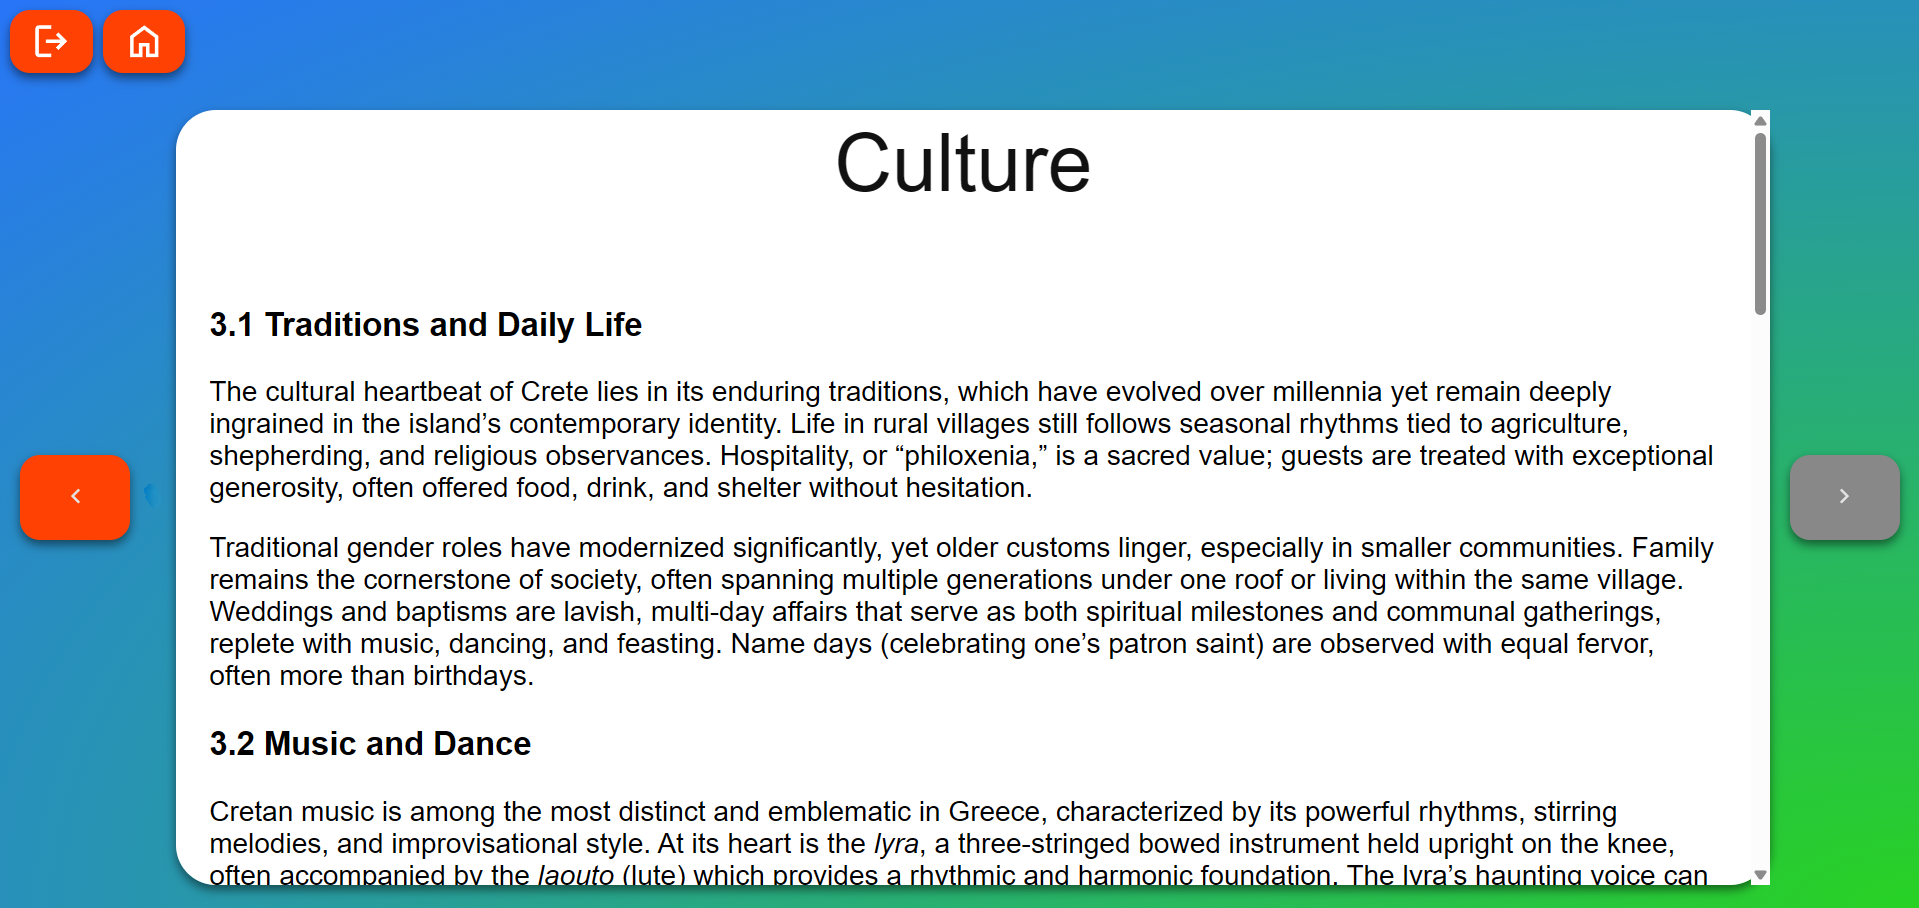
\includegraphics[width=0.5\linewidth]{img/Theory-Culture.png}
    \caption{\textlatin{Theory Chapters Page}}
\end{figure}

\newpage

\begin{itemize}
    \item Στο τέλος κάθε κεφαλαίου θεωρίας, ο χρήστης θα βρει ένα \textbf{κουμπί \textlatin{"Take the Quiz"}} το οποίο θα τον οδηγήσει στο αντίστοιχο \textlatin{\textbf{quiz}} γνώσεων του συγκεκριμένου κεφαλαίου που βρίσκεται και ολοκλήρωσε. (Κάθε κεφάλαιο έχει από ένα \textlatin{quiz} 15 ερωτήσεων, άρα συνολικά έχουμε 3 \textlatin{quizzes} και 45 διαφορετικές ερωτήσεις).
\end{itemize}
\begin{figure}[H]
    \centering
    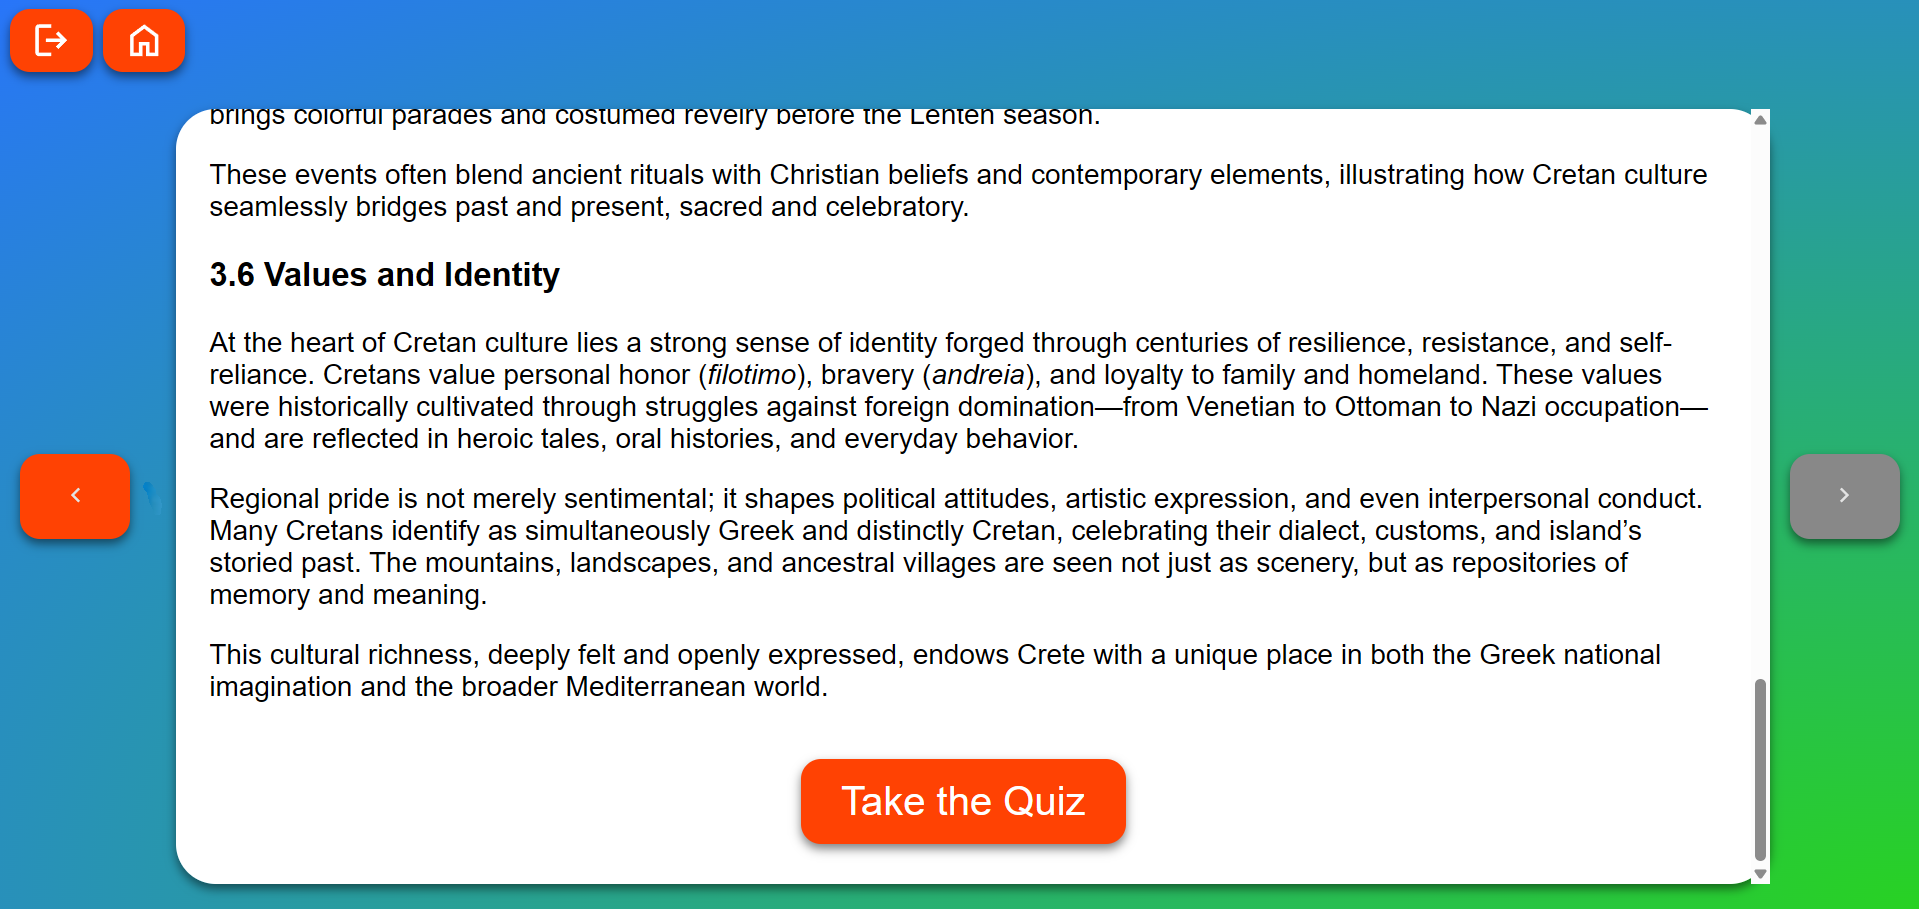
\includegraphics[width=1\linewidth]{img/Theory-TestButton.png}
    \caption{\textlatin{Theory Page-Quiz Button}}
\end{figure}
 
\bibliographystyle{alpha}
\bibliography{chrono_bibliography}